% -*- mode: latex-mode; TeX-engine: xetex; LaTeX-command-style: (("" "SOURCE_DATE_EPOCH=0 %(PDF)%(latex) --shell-escape %S%(PDFout)")); TeX-master: "../dissertation.tex"; -*-

\chapter{Two-photon Spectroscopy of NaCs Ground State}
\label{ch:raman-spectroscopy}

\section{Introduction}

\todo{make sure the goal of reaching the absolute ground state is stated previously.}

The excited molecular states measured and characterized in chapter \ref{ch:pa}
provide us a pathway to couple to the ground electronic molecular states
using two-photon transitions.
While it is in principle possible to drive from the atomic state
to any desired molecular ground state for various applications,
doing so directly has many technical challenges.
We will cover these challenges as well as the considerations in selecting
the molecule formation pathway in chapter \ref{ch:raman-transfer},
however, the difficulty, and the main difference from a pure atomic Raman transition,
lies in the wavefunction size mismatch.
As we have seen already in section \ref{pa:beampath},
the size mismatch between the excited molecular states and the ground atomic state
causes a very small FCF and requires a high PA intensity to improve the signal strength.
This small FCF also reduces the Rabi frequency for the two-photon transition to the ground state.
As a result, driving a two-photon transition to an arbitrary molecular ground state
may require maintaining coherence between two different lasers over
a relatively long time (milliseconds) which is very difficult to achieve.

Our solution to this challenge is to do the transfer via a two step process.
\begin{enumerate}
\item We drive a two-photon transition from the atomic state to
  a weakly bound ground state.
  The reduced energy difference allows the laser coherence to be maintained
  over a longer time easily.
  In the case of NaCs molecule, this also increases the FCF
  between the ground and excited molecular states which allows shorter pulse time and
  further reduces the coherence requirement.
\item The transfer to arbitrary molecular ground state will be done from
  the weakly bound state created in the first step.
  The strength of this transition can be much higher
  and only requires a relatively shorter laser coherence time.
  This step has already been demonstrated in other experiments\cite{ni_high_2008}
  so in this thesis we will focus only on the first step transfer.
\end{enumerate}

In this chapter, we will discuss the use of Raman spectroscopy
to measure the properties of the weakly bound molecular ground states.
In section \ref{ch:raman-spectroscopy:states}
we will describe the states involved and the setup for the Raman spectroscopy
as well as the measured binding energy for the $N=0$ states.
In section \ref{ch:raman-spectroscopy:n2}
we study the coupling between angular momentums for near threshold molecular states
by characterizing the $N=2$ states.

\section{Weakly Bound NaCs Ground States}
\label{ch:raman-spectroscopy:states}

As mentioned in section \ref{pa:structure:near-threshold},
the angular momentum coupling for weakly bound molecular state is similar to that of the atoms.
Therefore, instead of using the term symbol for the \textit{Hund's case (a)}
to identify the molecular potential and bound states,
we use the hyperfine state ($F_\Na, F_\Cs$) for the atoms instead.
Similarly, since the vibrational states of the molecule does not always corresponds to
a particular short range potential, we also label the vibrational states
from the the atomic state threshold.
Under this system, the atomic motional ground state is $v''=0$ and
the first (lowest binding energy) molecular bound state is $v''=-1$.

\todo{figure?}
In order to measure the binding energy of a molecular state,
we first prepare the atom in the corresponding hyperfine state
and drive a Raman transition to the molecular state.
We use a Raman transition that is detuned from the $c^3\Sigma\ v'=0$ state measured
in section \ref{pa:pa}.
When the Na and Cs are in the same tweezer,
they can undergo fast spin-exchange collision that changes the hyperfine state of the atom.
This process can cause the hyperfine energy ($>1~\mathrm{GHz}$) of the atoms
to be transferred to the motional energy
and eject the atoms from the tweezer ($<100~\mathrm{MHz}$ deep).
As a result, the measurement can only be done when the spin-exchange collision is suppressed,
which includes the following spin combinations,
\begin{enumerate}
\item $F_\Na=1$ and $F_\Cs=3$\\
  This is the spin state with the lowest energy and therefore the spin-exchange interaction
  is energetically forbidden.
  In the experiment, we use the state $|\mathrm{Na(1, 1),Cs(3, 3)}\rangle$
  which can be prepared from the $|\mathrm{Na(2, 2),Cs(4, 4)}\rangle$ state from OP
  easily by driving a Raman transition for both Na and Cs atoms.
  This state also remains the lowest energy atomic state in the present of a weak magnetic field.
\item $|\mathrm{Na(2, 2),Cs(4, 4)}\rangle$ and $|\mathrm{Na(2, 2),Cs(3, 3)}\rangle$
  \footnote{States with opposite $m_F$, i.e.
    $|\mathrm{Na(2, -2),Cs(4, -4)}\rangle$ and $|\mathrm{Na(2, -2),Cs(3, -3)}\rangle$ are also stable
    but are omitted here since these cannot be easily prepared in our experiment.}\\
  These spin states are stable because the spin-exchange collision conserves total $m_F$
  of the two atoms and
  the two states are the lowest energy states that has the same total $m_F$.
  Inelastic collision that changes the total $m_F$ can also happen
  but has a lower collision rate since it requires transferring angular momentum
  between the spin and motion of the atom.
\end{enumerate}

\subsection{Driving Raman Transition using the Optical Tweezer}

\begin{figure}
  \centering
  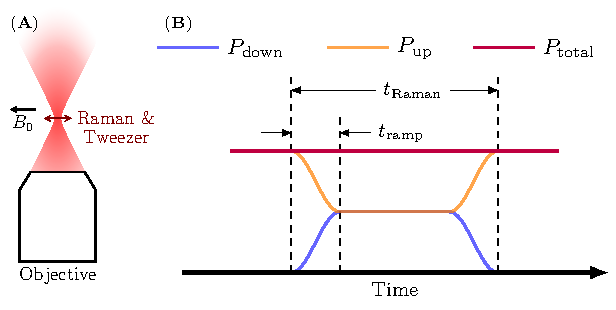
\includegraphics[width=\textwidth]{figures/raman_spectroscopy_apparatus_sequence.pdf}
  \caption[Raman transition setup and sequence]{
    (A) Geometry and polarization of trap and Raman beam relative to the bias magnetic field.
    We use a bias B field of $B_0=8.8~\mathrm{G}$ alone the tweezer polarization
    to define the quantization axis
    which is the same as the one used for Raman sideband cooling in Fig.~{fig:na-rsc-geometry}.
    As a result, the atoms experiences predominately $\pi$ polarization from the tweezer.
    (B) Raman transition pulse sequence.
    The tweezer initially consists of only up leg power.
    When driving the Raman transition, the up leg power is smoothly ramped down and
    the down leg power ramped up over $t_{\mathrm{ramp}}=10~\mathrm{\mu s}$
    while maintaining the total power of the tweezer.
    This minimizes the heating on the atoms due to power fluctuation while maximizes the time
    with maximum Raman Rabi frequency when the up and down leg powers are equal.
    \label{fig:raman-spectroscopy:apparatus-sequence}}
\end{figure}

\begin{figure}
  \centering
  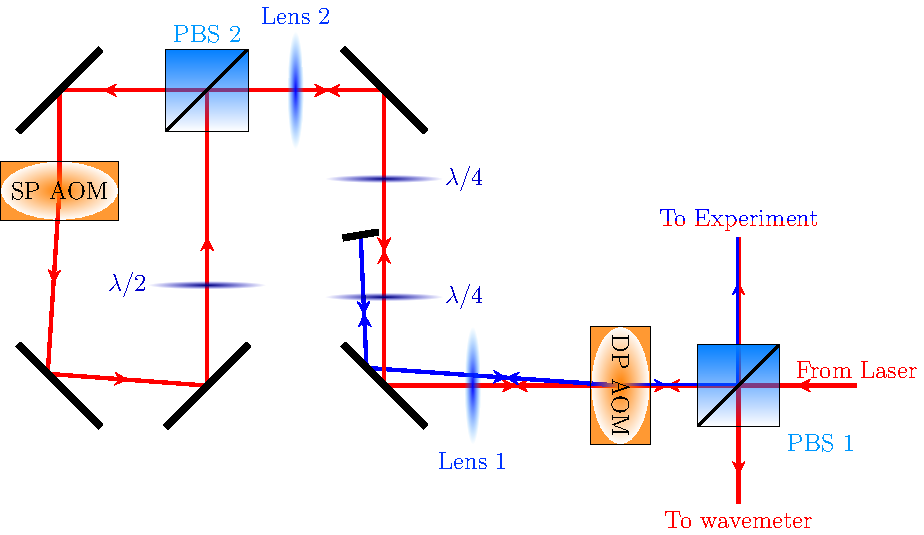
\includegraphics[width=\textwidth]{figures/raman_spectroscopy_raman_beampath.pdf}
  \caption[Beampath to allow driving Raman transition with tweezer]{
    Beampath for generating the frequency for Raman transition in the tweezer.
    (Beampath for fiber coupling and overall power control is not shown.)
    The red beam path is the $0$-th order of the double pass (DP) AOM
    which is used for the tweezer.
    When the DP AOM is turned on, some power is redirected to the first order
    (blue beam path) which generates the required frequency different to drive
    the Raman transition. The two frequencies are recombined on the DP AOM.
    The $0$-th order light is shifted by another single pass (SP) AOM
    running on a different frequency before recombining.
    Without this AOM, the leak light from the DP AOM will be at the same frequency
    as the $0$-th order light which can cause a significant power fluctuation
    due to interference. The SP AOM ensures that none of the leaking light frequency
    coincide with either intended frequencies therefore avoiding this issue.
    Different selection of the SP and DP AOM as well as their orders can be used
    to cover a wide range of two photon detuning for Raman transition.
    The experiment typically start with the SP AOM on and the DP AOM off.
    When driving the Raman transition, the powers on both AOMs are ramped simultaneously
    to achieve the desired power at both frequencies.
    \label{fig:raman-spectroscopy:raman-beampath}}
\end{figure}

In order to increase the intensity of the Raman beams to overcome the small FCF,
we use the tweezer beam to drive the Raman transition
(Fig.~\ref{fig:raman-spectroscopy:apparatus-sequence}A).
Not only does this maximizes the intensity due to the small focal size of the tweezer,
since the atoms are trapped at the maximum of the tweezer beam,
this also ensures that the Raman beam is aligned automatically to the atoms
and suppresses sensitivity to mechanical fluctuation that is usually
caused by a small beam size.
Moreover, this also minimizes the number of beams the atoms experience
during the Raman transition which, in turns, minimizes the scattering.
As a result, the coherence of the transition is also improved
which is important for achieving coherent creation of molecule
(chapter \ref{ch:raman-transfer}).

The beampath to generate the required frequencies in the tweezer is shown in
Fig.~\ref{fig:raman-spectroscopy:raman-beampath}.
The additional single pass AOM in the beampath avoids interference
with AOM leak light causing power fluctuation and
also increases the frequency tuning range compared to using only one double pass AOM.
The powers at each frequencies are calibrated as a function of AOM powers
so that we can select the desired power ratio during the experiment.
When driving the Raman transition, instead of turning on separate beam,
we ramp down the power at the original tweezer and ramping up the power
in the second frequency while maintaining the total power to minimize heating of the atoms
(Fig.~\ref{fig:raman-spectroscopy:apparatus-sequence}B).

\subsection{Raman Resonance on $N=0$ Ground State}
\label{ch:raman-spectroscopy:n0}

\begin{figure}
  \centering
  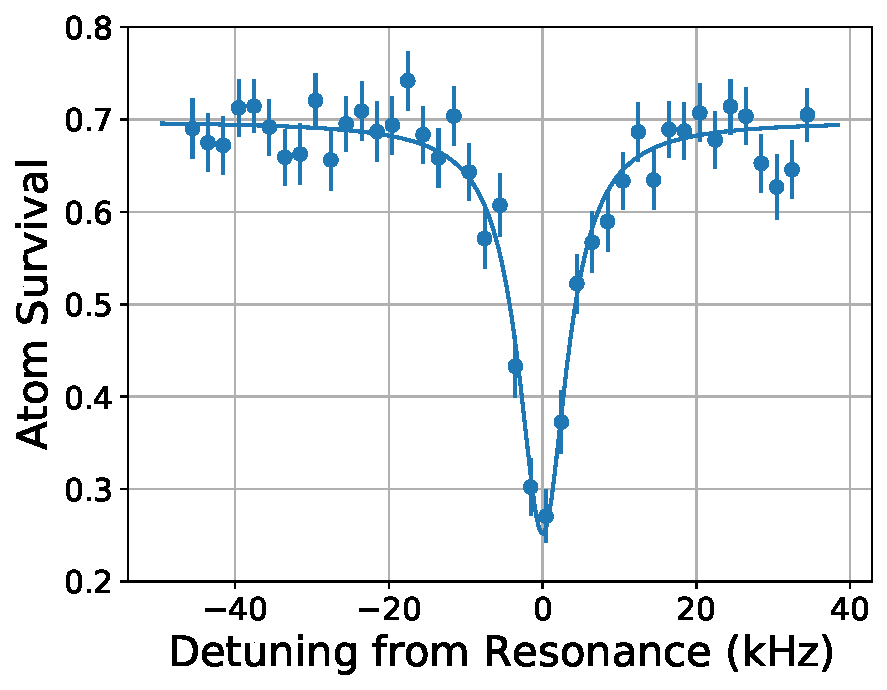
\includegraphics[width=0.7\textwidth]{figures/raman_spectroscopy_resonance.pdf}
  \caption[Raman resonance for $v''=-1,\ N=0$ state]{
    Raman resonance for $v''=-1,\ N=0$ state from $|\mathrm{Na(2, 2),Cs(4, 4)}\rangle$.
    \label{fig:raman-spectroscopy:resonance}}
\end{figure}

\begin{table}
  \centering
  \todo{include theory prediction?}
  \begin{tabular}{|c|c|c|c|}
    \hline
    \multirow{2}{*}{Spin state}&\multicolumn{2}{c|}{Resonance (MHz)}&\multirowcell{2}{Zeeman shift\\(kHz/G)}\\\cline{2-3}
    {}&$8.8~\mathrm{G}$&$0~\mathrm{G}$&\\\hline
    $|\mathrm{Na(2, 2),Cs(4, 4)}\rangle$&$297.8472(28)$&$297.8510(28)$&$-0.43(10)$\\\hline
    $|\mathrm{Na(1, 1),Cs(3, 3)}\rangle$&$367.7892(25)$&$369.63(29)$&$-209(33)$\\\hline
    $|\mathrm{Na(2, 2),Cs(3, 3)}\rangle$&$770.200516(24)$&$769.8294(22)$&$42.17(24)$\\\hline
  \end{tabular}
  \caption[Binding energies for $v''=-1,\ N=0$ states]{
    Binding energies and Zeeman shift for $v''=-1,\ N=0$ states.
    \label{table:raman-spectroscopy:n0}}
\end{table}

We first measure the binding energy for the $v=''-1,\ N=0$ state
from the atomic states $|\mathrm{Na(2, 2),Cs(4, 4)}\rangle$, $|\mathrm{Na(1, 1),Cs(3, 3)}\rangle$,
and $|\mathrm{Na(2, 2),Cs(3, 3)}\rangle$.
\todo{theory prediction?}
Fig.~\ref{fig:raman-spectroscopy:resonance} shows the measured Raman resonance from
$|\mathrm{Na(2, 2),Cs(4, 4)}\rangle$ using $10~\mathrm{mW}$ of tweezer power at a detuning of
$-100~\mathrm{GHz}$ from the $v'=0$ excited state and a $2~\mathrm{ms}$ pulse time.

The tweezer also shifts the resonance frequency.
We remove this effect by measuring the resonance at different tweezer power
and extrapolate to zero trap powers.
Similarly, we measure the Zeeman shift and the resonance frequency at zero magnetic field.
The summary of the results are shown in table~\ref{table:raman-spectroscopy:n0}.

\begin{figure}
  \centering
  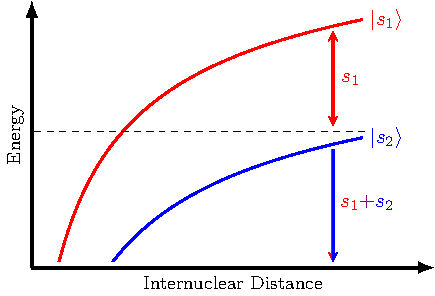
\includegraphics[width=0.7\textwidth]{figures/raman_spectroscopy_spin_mixing.pdf}
  \caption[Spin state mixing near the atomic threshold.]{
    Spin state mixing near the atomic threshold.
    Energy above the $s_2$ threshold only supports one molecular spin state
    so the bound state within the $s_1$ potential in this region is
    almost purely $s_1$.
    Energy below the $s_2$ threshold supports both $s_1$ and $s_2$ molecular states
    so bound states in this region may have a mixture of $s_1$ and $s_2$
    if the two spin states are coupled.
    This includes all the $s_2$ bound states and some of the $s_1$ bound states.
    \label{fig:raman-spectroscopy:spin-mixing}}
\end{figure}

Note that the Zeeman shift for the $|\mathrm{Na(2, 2),Cs(4, 4)}\rangle$ state
is signicantly smaller than that for other spin states.
The reason for this is spin mixing due to magnetic coupling between states
with the same total $m_F$\footnote{The same coupling that leads to spin exchange collision.}.
The $|\mathrm{Na(2, 2),Cs(3, 3)}\rangle$ spin state is coupled to the
$|\mathrm{Na(2, 2),Cs(4, 3)}\rangle$, $|\mathrm{Na(1, 1),Cs(4, 4)}\rangle$
and $|\mathrm{Na(2, 1),Cs(4, 4)}\rangle$ states
whereas $|\mathrm{Na(1, 1),Cs(3, 3)}\rangle$ is coupled to the
$|\mathrm{Na(2, 1),Cs(3, 3)}\rangle$, $|\mathrm{Na(1, 1),Cs(4, 3)}\rangle$,
$|\mathrm{Na(2, 1),Cs(4, 3)}\rangle$, $|\mathrm{Na(2, 2),Cs(3, 2)}\rangle$
and $|\mathrm{Na(2, 2),Cs(4, 2)}\rangle$ states.
All of these states listed above has higher energy so their bound states
may cause spin mixing with the $|\mathrm{Na(2, 2),Cs(3, 3)}\rangle$ and
$|\mathrm{Na(1, 1),Cs(3, 3)}\rangle$ bound states (Fig.~\ref{fig:raman-spectroscopy:spin-mixing})
causing them to have a different magnetic field dependency from the corresponding atomic state
resulting in a non-zero differential Zeeman shift.
On the other hand, the $|\mathrm{Na(2, 2),Cs(4, 4)}\rangle$ bound state is above
all the other spin states and therefore has a mostly pure spin state
and the transition has little Zeeman shift.

\section{Rotational Excited NaCs Ground State}
\label{ch:raman-spectroscopy:n2}

In additional to the $N=0$ state, we also measure the energies of rotational excited states.
Not only do these measurements allow us to verify the rotational state for our previous results,
we can also take advantage of the precision of the Raman spectroscopy
to study the rich interaction between the nuclear rotation and atomic spin.

Due to parity conservation in the Raman transition,
the final molecular state must have an even $N$
so the lowest rotational excited state we can address is $N=2$.
We use $|\mathrm{Na(2, 2),Cs(4, 4)}\rangle$ as the initial state since,
as we saw in the previous section, the corresponding molecular bound state
has the least mixing other molecular potentials.
Similarly, we select $F_{\mathrm{atom}}=6$ as the final total atomic spin state
since this is the state we address in the corresponding $N=0$ spectroscopy and
it includes the $m_{F_{\mathrm{atom}}}=6$ state which has minimum
Zeeman shift as discussed in the previous section.

\subsection{Angular Momentum Coupling in $N=2$ Ground State}

Since the full Hamiltonian is rotaionally symmetric for rotation around the field direction,
$m_F\equiv m_{F_{\mathrm{atom}}}+m_{N}=6$ is conserved in the Raman transition,
which includes a total of three states.
However, the exact states we are coupling to and the good quantum numbers depends on
the strength of the external field.

At zero or very low external field, the good quantum numbers are $F$ and $m_F$
due to coupling between $\mathbf{F}_{\mathrm{atom}}$ and $\mathbf{N}$.
as discussed in section \ref{pa:structure:near-threshold}.
In this basis, the three energy eigenstates are
$|F=6,m_F=6\rangle$, $|F=7,m_F=6\rangle$ and $|F=8,m_F=6\rangle$.

External field, both magnetic and electric\footnote{Light field from the tweezer.},
couples mostly to the atomic spin $\mathbf{F}_{\mathrm{atom}}$
\footnote{More precisely the electron spin within $\mathbf{F}_{\mathrm{atom}}$.}
rather than the nuclear rotation $\mathbf{N}$.
Therefore, at high field $\mathbf{F}_{\mathrm{atom}}$ and $\mathbf{N}$
decouples and their projections become good quantum numbers individually.
In this case, the three energy eigenstates are
$|m_{F_\mathrm{atom}}=6,m_N=0\rangle$, $|m_{F_\mathrm{atom}}=5,m_N=1\rangle$ and
$|m_{F_\mathrm{atom}}=4,m_N=2\rangle$.

\subsection{$N=2$ Raman Resonances}

\begin{figure}
  \centering
  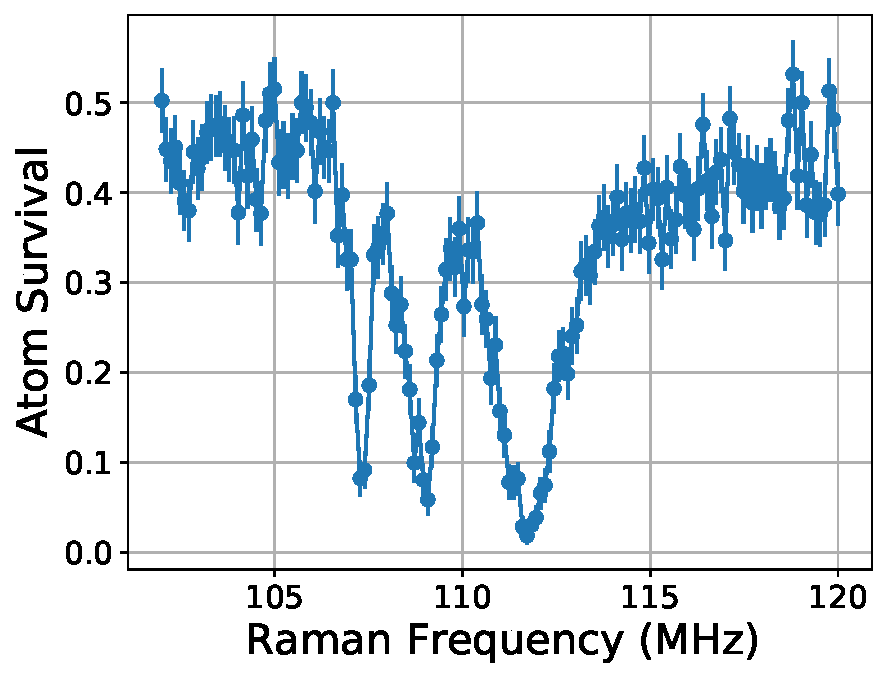
\includegraphics[width=0.7\textwidth]{figures/raman_spectroscopy_n2_resonance.pdf}
  \caption[$N=2$ Raman spectrum.]{
    $N=2$ Raman spectrum with $8.8~\mathrm{G}$ of magnetic field
    and $10~\mathrm{mW}$ of tweezer power.
    The three resonances corresponds to three $m_F=6$ states.
    \label{fig:raman-spectroscopy:n2}}
\end{figure}

Fig.~\ref{fig:raman-spectroscopy:n2} shows the Raman spectrum taken
at $8.8~\mathrm{G}$ of magnetic field and $10~\mathrm{mW}$ of tweezer power
where three resonances can be clearly seen as expected.
This single measurement, however, does not allow us to directly identify the states
that correspond to each of the resonances.
Because of this, we measured the resonance at various tweezer powers and magnetic field
as shown in Fig.~\ref{fig:raman-spectroscopy:n2-fit}.
Each dot in the plot corresponds to an observed resonance frequency.

\begin{figure}
  \centering
  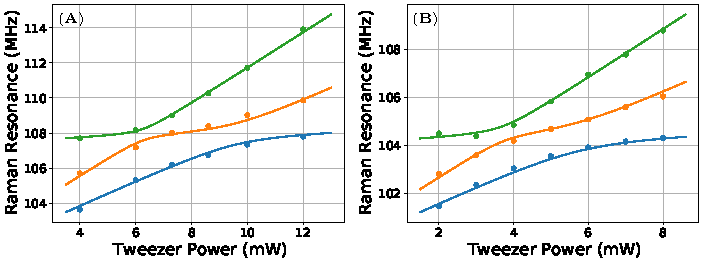
\includegraphics[width=\textwidth]{figures/raman_spectroscopy_n2_fit.pdf}
  \caption[$N=2$ Raman resonances and fitting to external field strengths.]{
    Dependency of $N=2$ Raman resonances on the tweezer power at
    (A) $8.8~\mathrm{G}$ and (B) $5.28~\mathrm{G}$ magnetic field.
    The different colors shows the resonance frequency for the states with
    the lowest (blue), second lowest (orange) and highest (green) binding energies.
    All of the data are taken in the intermediate field regime
    and therefore in a mixture of different spin states.
    The lines are fits to the resonance frequencies using a field dependent Hamiltonian.
    \label{fig:raman-spectroscopy:n2-fit}}
\end{figure}

\begin{table}
  \centering
  \begin{tabular}{|@{}c@{}|}
    \hline
    $H_0$ parameters\\\hline
    \begin{tabularx}{0.7\textwidth}{Y|Y|Y|Y}
      $E_0$ (MHz)&$\Delta E_6$ (MHz)&$\Delta E_7$ (MHz)&$\Delta E_8$ (MHz)\\\hline
      $-99.196(89)$&$-0.146(87)$&$-0.652(78)$&$0.80(11)$
    \end{tabularx}\\\hline
    AC Stark shift parameters\\\hline
    \begin{tabularx}{0.7\textwidth}{Y|Y|Y}
      $a_0$ (MHz/mW)&$a_1$ (MHz/mW)&$a_2$ (MHz/mW)\\\hline
      $1.015(18)$&$0.721(21)$&$6.4(22)\times10^{-2}$
    \end{tabularx}\\\hline
    Zeeman shift parameters\\\hline
    \begin{tabularx}{0.7\textwidth}{Y|Y|Y}
      $b_0$ (MHz/G)&$b_1$ (MHz/G)&$b_2$ (MHz/G)\\\hline
      $-0.237(22)$&$-0.222(22)$&$-0.947(23)$
    \end{tabularx}\\\hline
  \end{tabular}
  \caption[$N=2$ effective Hamiltonian parameters.]{
    Fitted parameters for the $N=2$ Hamiltonian. Since the $\Delta E_F$s are not independent
    $\Delta E_8$ is not a free parameter and is rather $-\Delta E_6-\Delta E_7$.
    Also note that the fit is directly from the binding energy measured
    in Fig.~\ref{fig:raman-spectroscopy:n2-fit} so the zero energy of the Hamiltonian is
    the atomic $|\mathrm{Na(2, 2),Cs(4, 4)}\rangle$ state
    which also has non-zero Zeeman an AC Stark shifts.
    \label{table:raman-spectroscopy:n2}}
\end{table}

In order to understand the dependency of the resonances on the external fields
we use the following phenomenological model.
The Hamiltonian in the $m_F=6$ subspace we coupled to can be expressed as,
\begin{align*}
  H=&H_0+H_1
\end{align*}
where $H_0$ is the zero field term due to the coupling
between $\mathbf{F}_{\mathrm{atom}}$ and $\mathbf{N}$,
and the $H_1$ term is due to the coupling to external fields.
At zero external field, the eigenstates are the $F$ and $m_F$ basis
and the most generic term is,
\begin{align*}
  H_0=&E_0+\!\!\sum_{F=6,7,8}\Delta E_F|F,m_F=6\rangle\langle F,m_F=6|
\end{align*}
where $E_0$ is the ``average'' energy and $\Delta E_F$ are the shift for each $F$ states
with $\sum_{F=6,7,8}\Delta E_F = 0$.
The term for coupling to the external fields couples to the $m_{F_\mathrm{atom}},m_N$ basis
and the generic expression for such a term is,
\begin{align*}
  H_1=&\sum_{i=0,1,2}\paren{P_{\mathrm{tweezer}}\cdot a_i+B\cdot b_i}|m_{F_\mathrm{atom}}=6-i,m_N=i\rangle\langle m_{F_\mathrm{atom}}=6-i,m_N=i|
\end{align*}
where $P_{\mathrm{tweezer}}$ is the tweezer power, $B$ is the magnetic field,
and $a_i$ and $b_i$ are the state dependent AC Stark shift and Zeeman shift
of the binding energies.
We numerically diagnolize this Hamiltonian and fit to the experimental data
as shown in the lines in Fig.~\ref{fig:raman-spectroscopy:n2-fit}.
The free parameters of the Hamiltonian we obtained are shown in
table~\ref{table:raman-spectroscopy:n2}.

\section{Summary and Outlook}
\todo{}
